\section{平台实现和评估}\label{sec:implimentation-evaluation}

\subsection{平台实现}

我们实现了\cref{sec:overview}中所述的设计,受限于工程能力和时间,我们对一些不重要但比较复杂的部分进行了简化,重点是使实现的平台能够表达出一个简单但接近真实的场景,以此说明设计的安全性和合理性,并方便对性能进行初步测试。% 我们的实现除了已有的开源代码,共包含约

\paragraph{运行时实现}

由于本次设计的微服务示例程序用到的操作系统支持很少,因此我们在Graphene-SGX~\cite{tsai2017graphene}的基础上删掉了大部分操作系统的特性,只保留了能够支持微服务运行的最小功能,包括网络通信、内存管理、远程验证等,由此作为运行时实现。
% 我们将这个运行时实现命名为Graphene-SGX-Micro,它的代码量约为Graphene-SGX的1/10。

\paragraph{远程验证协议实现}

对于向SGX IAS请求远程验证,Graphene-SGX中已实现了该功能,因此不用进行实现。但我们将其与其他SGX相关功能封装为一个模块,方便其他模块使用。

另外我们分别实现了DHKE、对称加密、信任白名单T等模块,结合Rust的TCP库,按照之前设计的协议流程,实现了一个简单的安全通信协议。实现的形式为一个Rust crate,可以作为函数库供程序进行链接与使用。

在通信的检查部分,为了方便实现,2层检查并没有采用并行的方式,而是按照顺序依次进行。对于信任白名单T,我们在哈希Map的基础上实现;为防止其他微服务地址变化导致表中记录弃用,占用过多内存,我们适当限制了T的大小,并使用最近最少使用(LRU)算法清理弃用项。
% 因为实现一个完整的通信协议库需要考虑很多细节(例如OpenSSL~\cite{openssl}),而本次实现不着重讨论这些细节,因此不能保证库的实现是安全的,不能用于生产场景。

\paragraph{微服务示例实现}

我们按照\cref{subsec:ms-example}中的微服务设计,使用Rust的gRPC库Tonic~\cite{tonic}实现了除数据持久化节点之外的所有微服务节点,并使用jsonwebtoken库生成和验证JWT,用来实现基于Token交换的授权机制。数据持久化节点暂时使用开源的Redis~\cite{redis}进行模拟。

为了进行测试,我们还实现了一个简单的客户端程序,用来模拟用户的请求。为简化处理,客户端和API网关之间的通信也使用了gRPC协议,而不是客户端和服务端交互下更常用的HTTP协议。

\subsection{评估}

\textbf{实验环境:}我们在3台拥有Intel E3-1280 V6 CPU、64GB内存、支持SGX v1的服务器上运行程序和进行实验。其中1台机器运行Ubuntu 22.04操作系统,内核版本为5.15.0-56-generic;另外两台运行Ubuntu 16.04,内核版本为4.4.0-210-generic和4.4.0-176-generic。我们在3台机器上分别配置了SGX内和SGX外的运行环境,在Ubuntu 22.04系统的机器上运行各微服务程序,在另外两台机器上分别运行API网关和客户端程序,由此进行实验评估。

\subsubsection{性能表现}

由于其他相关工作都没有开源实现,且侧重点有所区别,因此我们的工作聚焦于比较微服务示例程序在SGX内外的通信和计算性能表现。

为了比较不同运行环境和通信协议下的性能,以及比较不同类型微服务的性能,我们将微服务示例程序分别在SGX外的Linux系统和SGX内的运行时内运行,在64*64、128*128、256*256、512*512、1024*1024和2048*2048共6种不同尺寸的标准测试图片上分别测试了灰度图服务、模糊图服务和字符画服务,每种情况测试20次,分别记录用户端总用时、API网关总用时和微服务节点用时,由此计算出用户端和API网关的端到端通信往返时间、API网关和微服务节点的端到端通信往返时间以及微服务节点的处理时间,并计算得到平均值,得到的结果如图\ref{fig:evaluation}所示。

\begin{figure}[!ht]
    \centering
    \begin{subfigure}{0.96\textwidth}
        \centering
        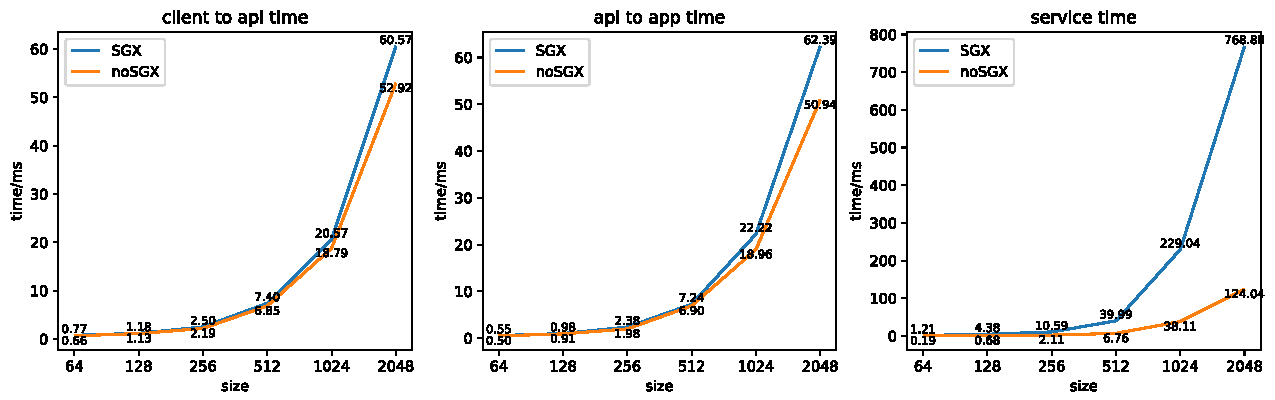
\includegraphics[width=\textwidth]{figures/grayscale.pdf}
        \caption{灰度图服务}
    \end{subfigure}
    \begin{subfigure}{0.96\textwidth}
        \centering
        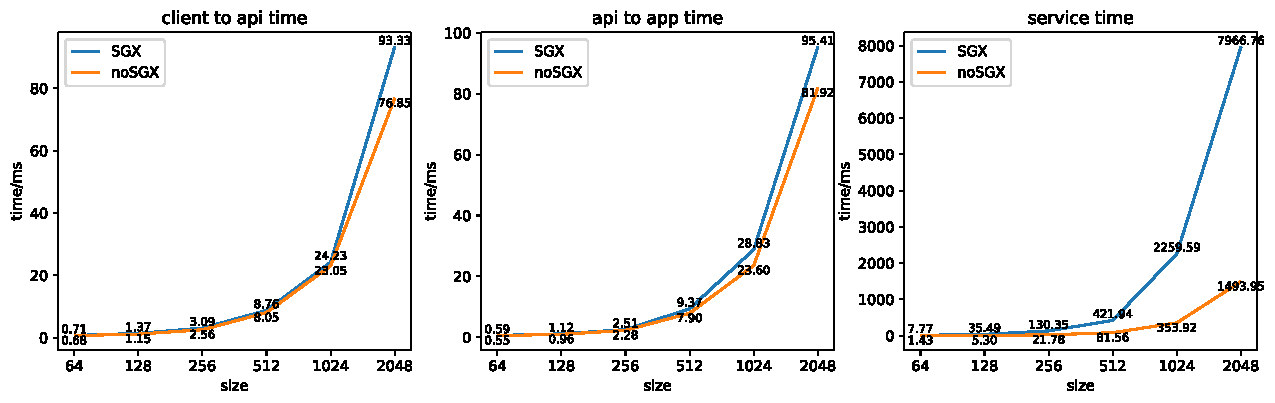
\includegraphics[width=\textwidth]{figures/blur.pdf}
        \caption{模糊图服务}
    \end{subfigure}
    \begin{subfigure}{0.96\textwidth}
        \centering
        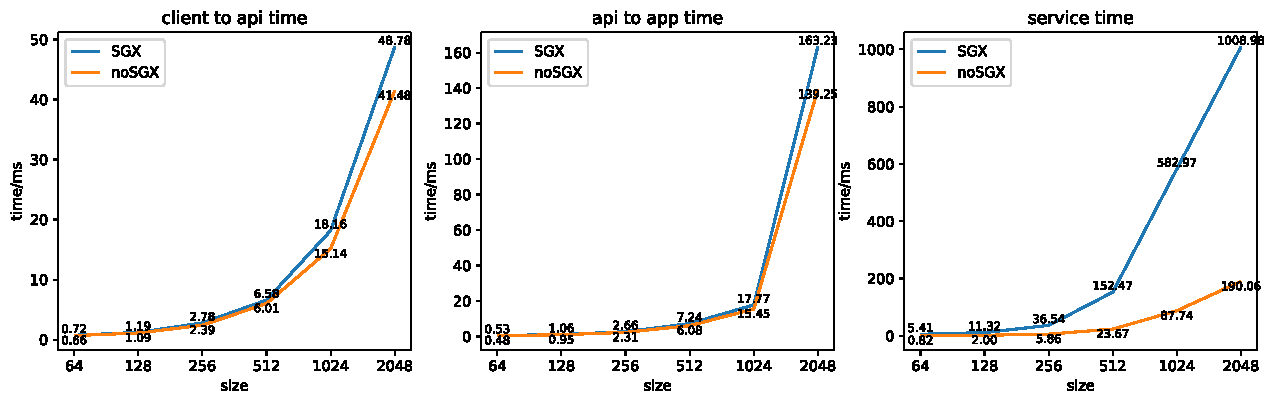
\includegraphics[width=\textwidth]{figures/ascii.pdf}
        \caption{字符画服务}
    \end{subfigure}
    \caption{SGX内外不同微服务通信和计算耗时}
    \label{fig:evaluation}
\end{figure}

我们可以看到,在三种不同的微服务中,随着图片尺寸的增大,在SGX内外运行的微服务程序通信延迟都相应增大,但是相差较小,在SGX中运行的微服务节点间的通信带来了额外的约14.3\%的延迟,推测是数据进出SGX飞地时加解密造成的;但是由于网络通信的主要开销来自于网络包的传递,因此二者差别较小,相比于SGX提供的安全保障,这些延迟是可以接受的。而在计算性能方面,SGX内的运行时带来了4.79-7.56倍的计算开销,这一较大的开销与我们对Graphene-SGX和Rust-SGX的测试是相符合的,对于微服务计算的场景来说需要通过进一步的研究来降低。

对于不同微服务之间的通信和计算开销的比较,我们发现通信开销中字符画服务最小,而模糊图服务最大。原因是字符画服务会经过裁剪,输出数据量是最小的;而模糊图服务经过模糊处理后图像压缩比会下降,导致输出的数据量最大。对于计算开销,灰度图服务最小,而模糊图服务最大。原因是灰度图服务只需要进行简单的灰度转换,计算简单;而模糊图服务基于高斯模糊(Gaussian blur)算法,需要进行卷积操作,计算开销最大。

对于字符画服务,由于其还要与调整大小服务和灰度图服务进行通信,且因为调整图片大小导致数据量变化,因此我们对其进行了更细致的分析,将字符画服务处理时间细分为解码图片、与调整大小微服务通信、调整大小微服务处理、与灰度图微服务通信、灰度图微服务处理、字符画微服务计算共6个部分,得到了如图\ref{fig:evaluation-ascii}所示的结果。

\begin{figure}[!ht]
    \centering
    \begin{subfigure}{0.3\textwidth}
        \centering
        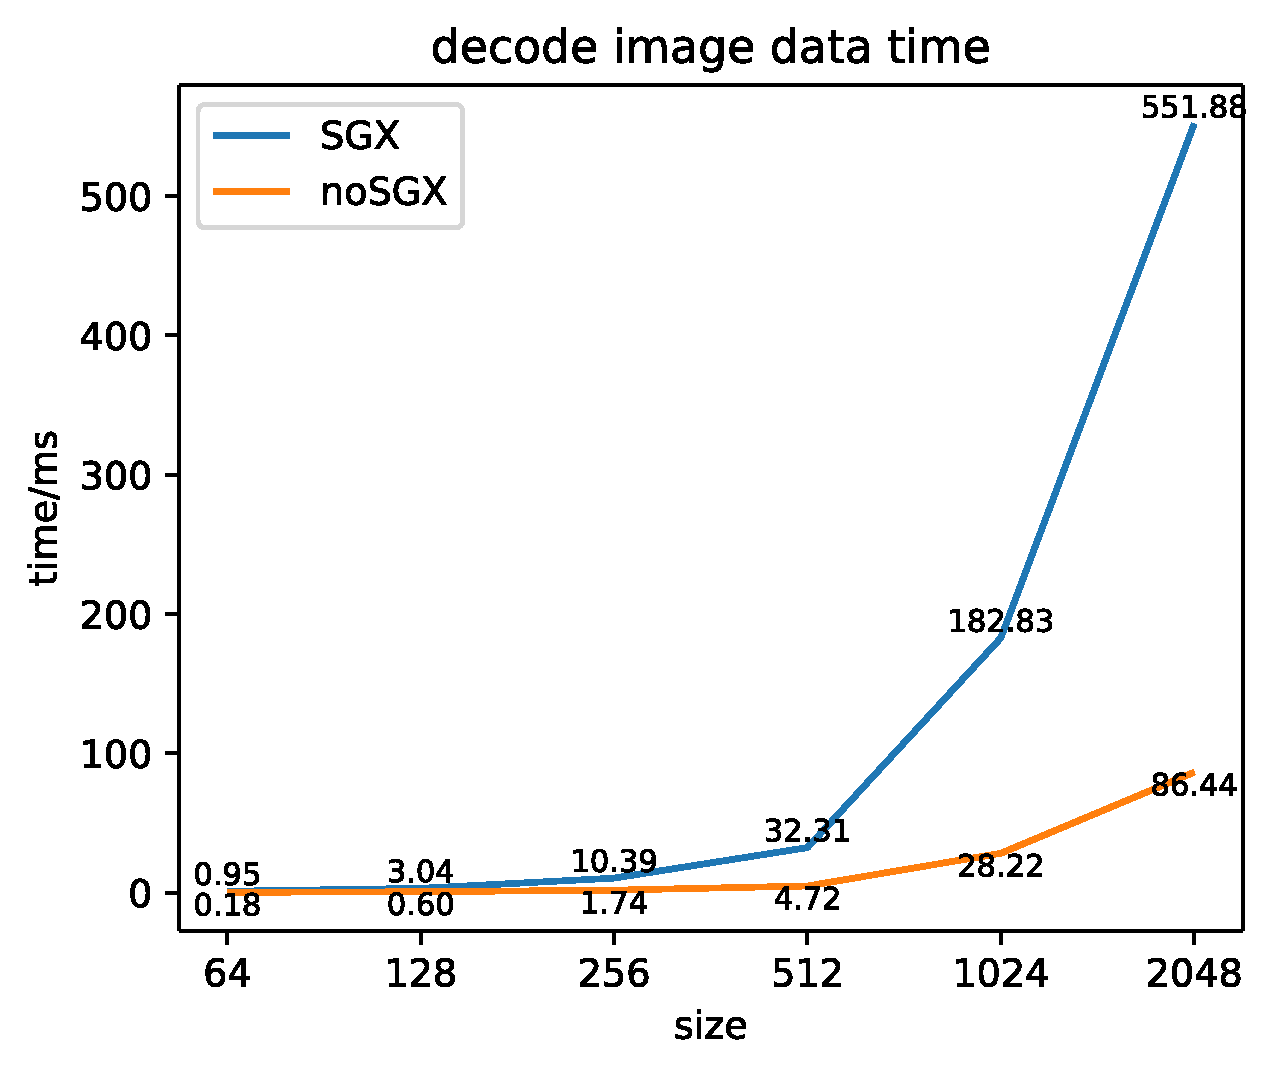
\includegraphics[width=\textwidth]{figures/decode_image.pdf}
        \caption{解码图片}
    \end{subfigure}
    \begin{subfigure}{0.3\textwidth}
        \centering
        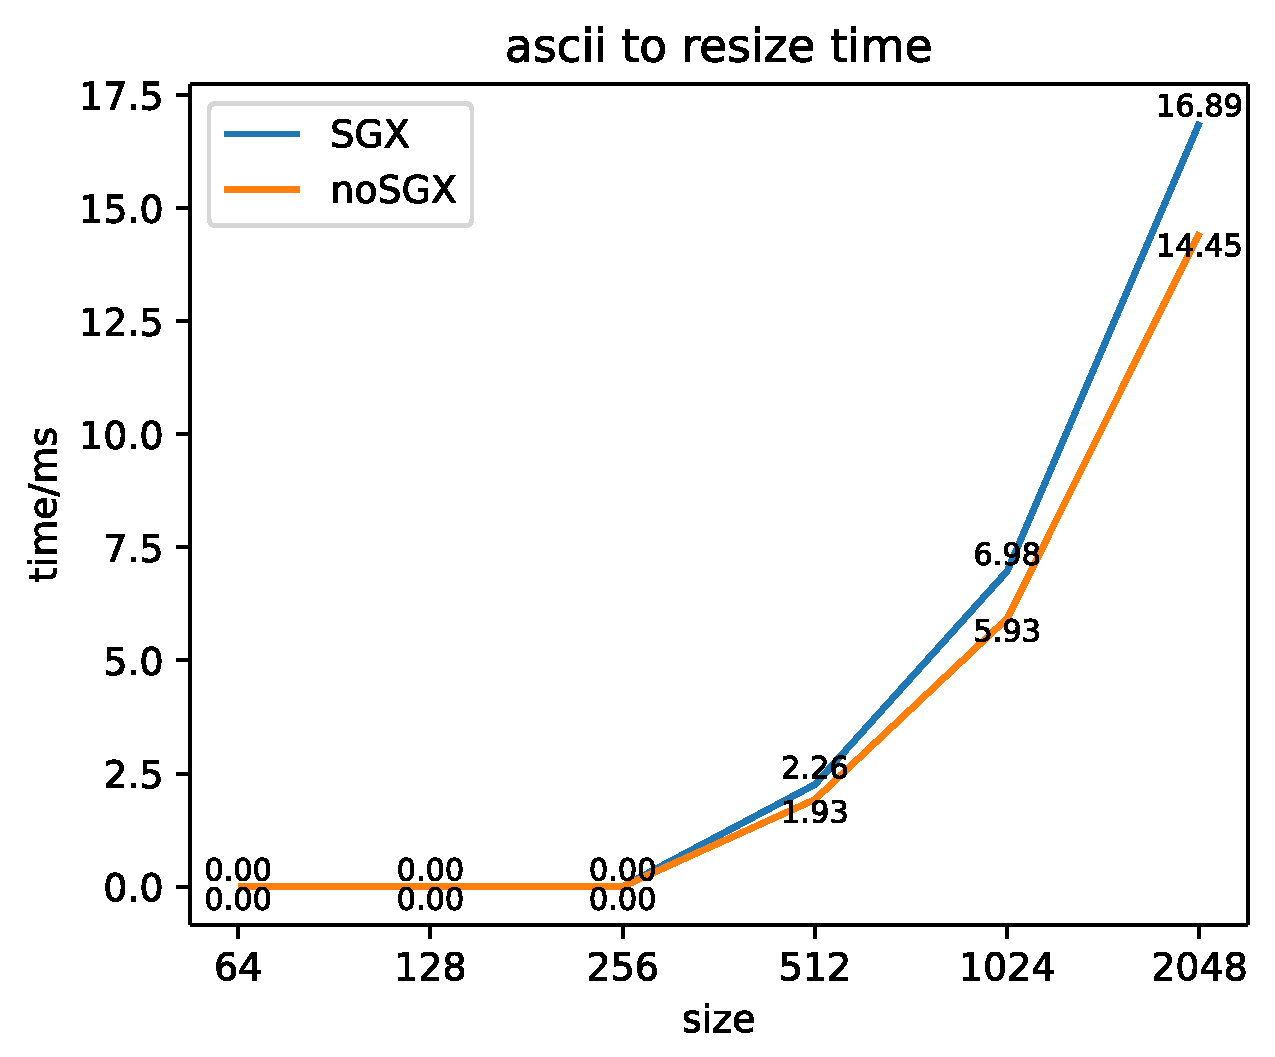
\includegraphics[width=\textwidth]{figures/ascii_to_resize.pdf}
        \caption{与调整大小微服务通信}
    \end{subfigure}
    \begin{subfigure}{0.32\textwidth}
        \centering
        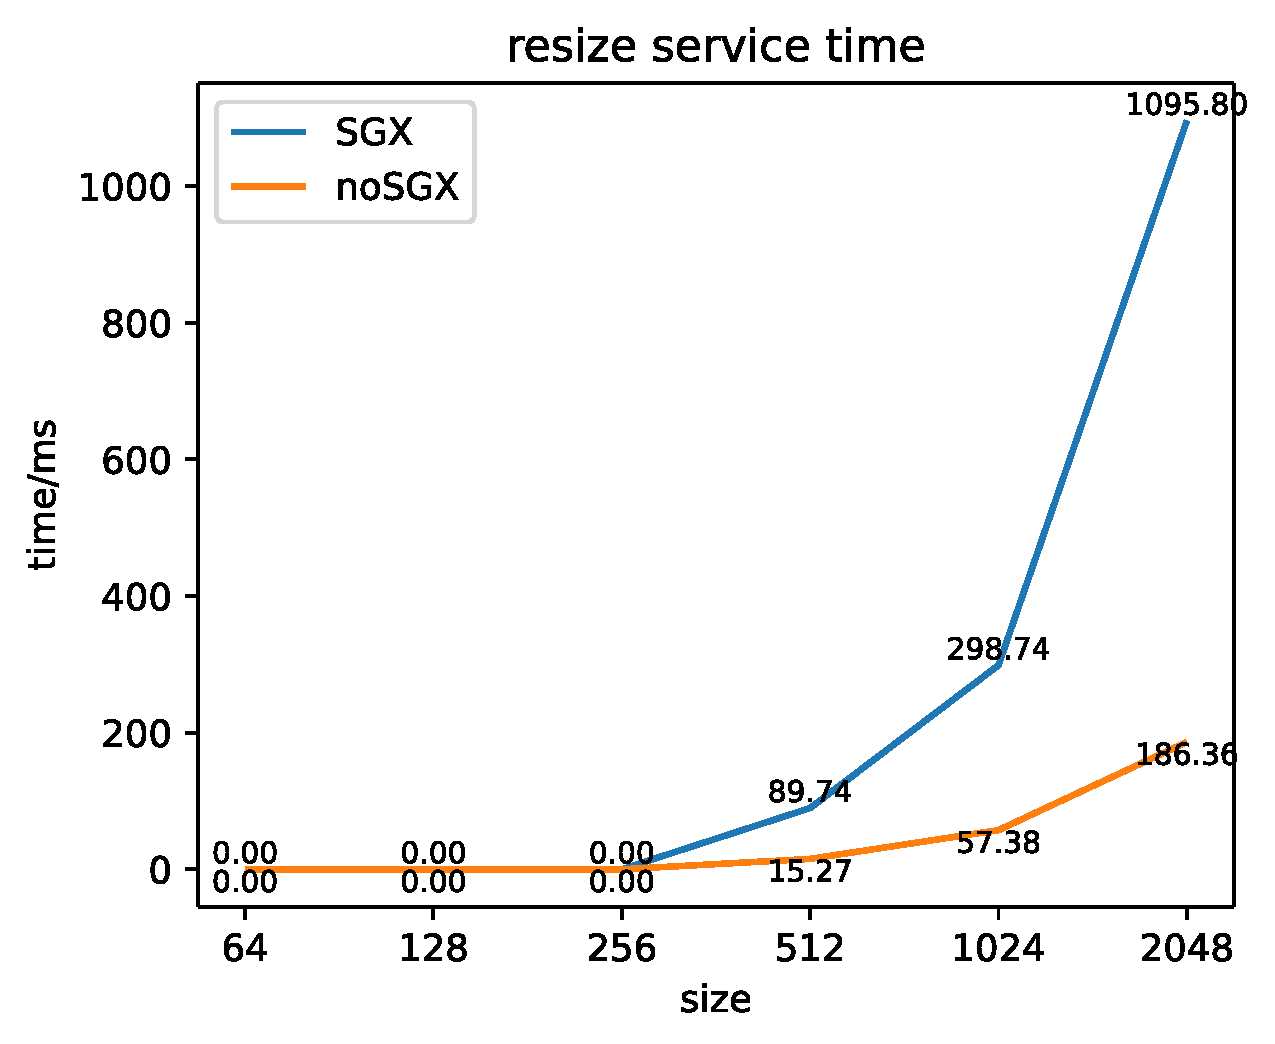
\includegraphics[width=\textwidth]{figures/resize_service.pdf}
        \caption{调整大小微服务处理}
    \end{subfigure}
    \begin{subfigure}{0.32\textwidth}
        \centering
        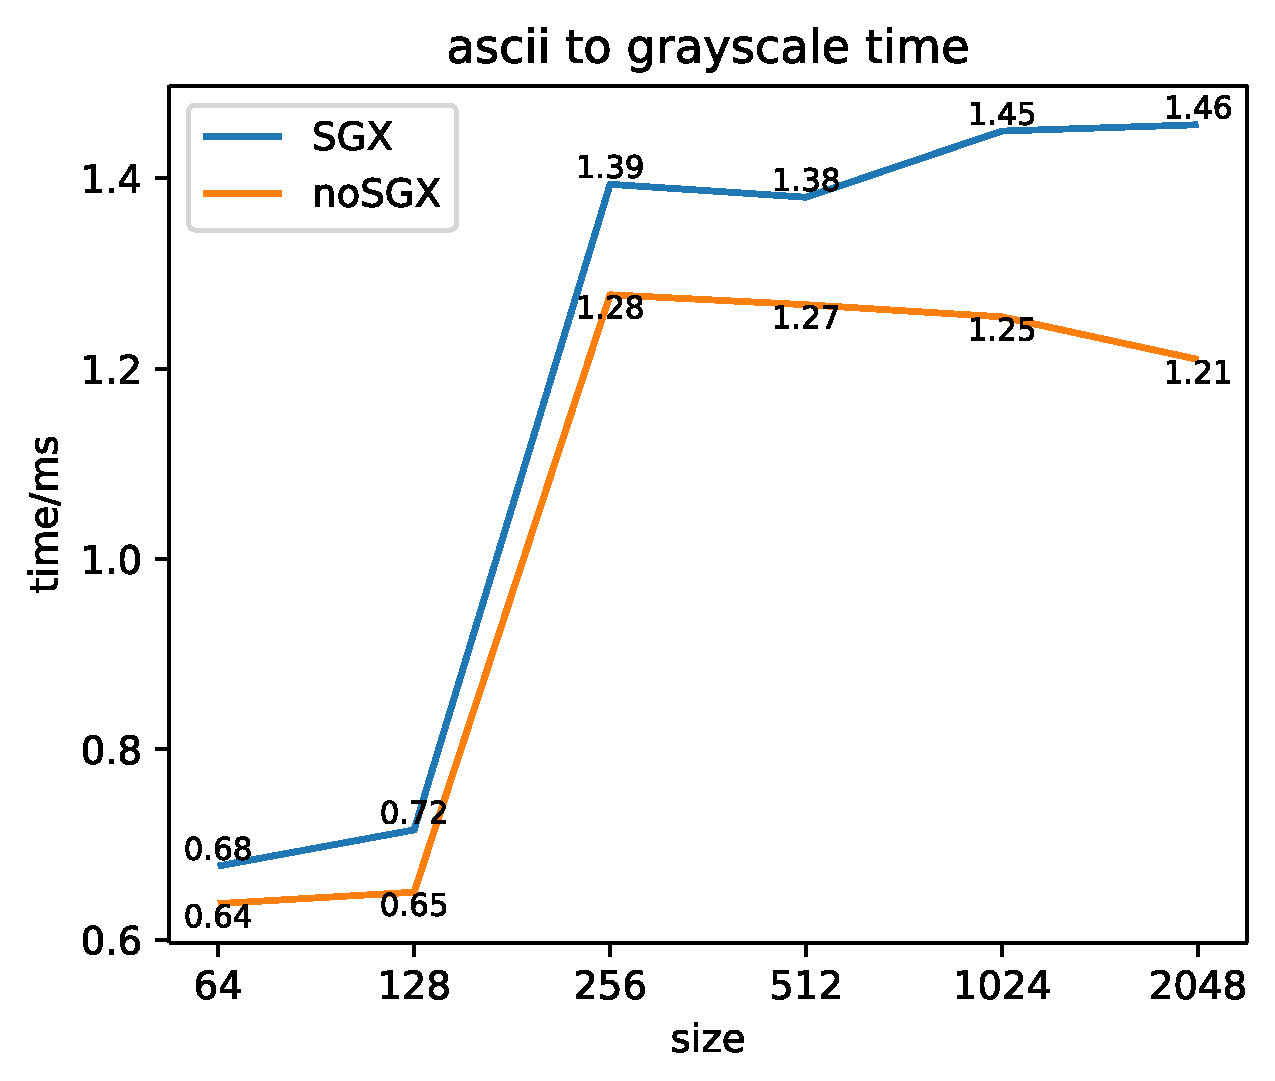
\includegraphics[width=\textwidth]{figures/ascii_to_grayscale.pdf}
        \caption{与灰度图微服务通信}
    \end{subfigure}
    \begin{subfigure}{0.32\textwidth}
        \centering
        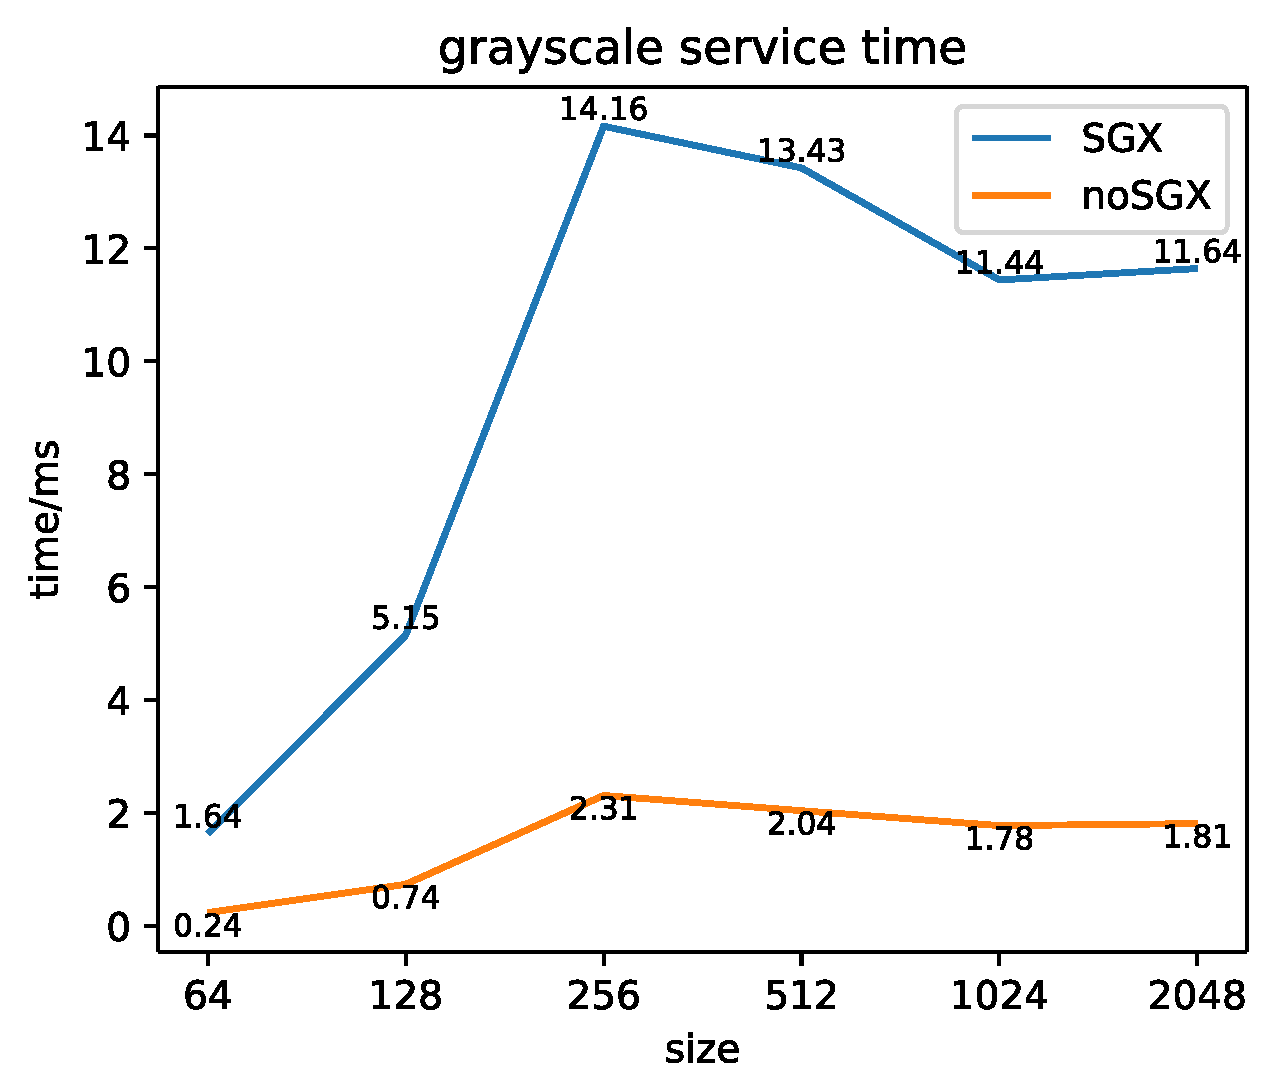
\includegraphics[width=\textwidth]{figures/grayscale_service.pdf}
        \caption{灰度图微服务处理}
    \end{subfigure}
    \begin{subfigure}{0.32\textwidth}
        \centering
        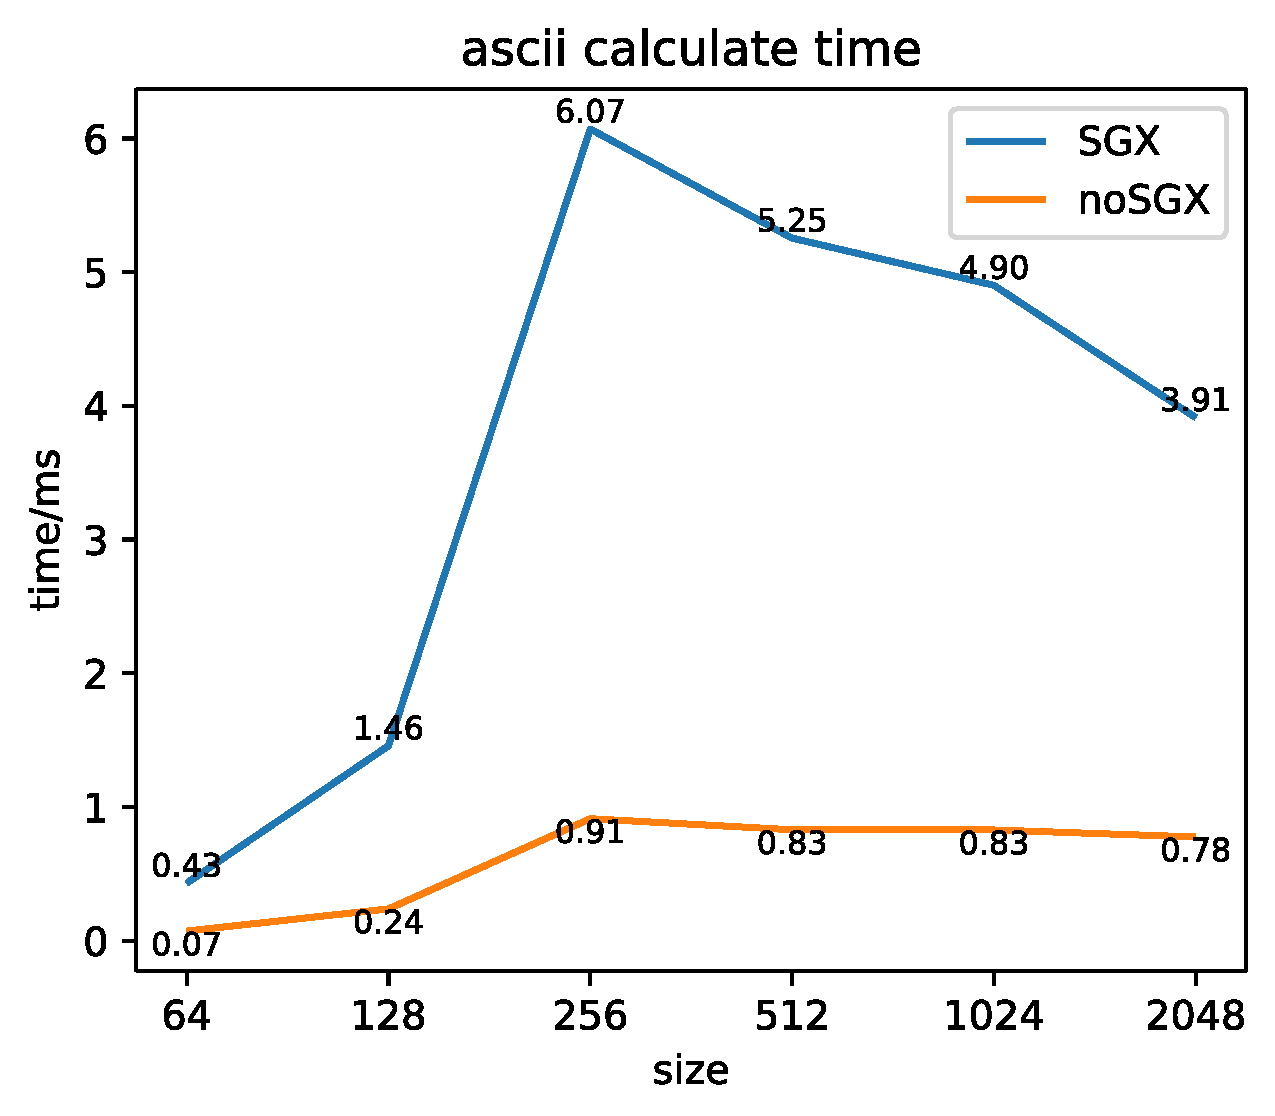
\includegraphics[width=\textwidth]{figures/ascii_cal.pdf}
        \caption{字符画微服务计算}
    \end{subfigure}
    \caption{字符画微服务处理各部分时间}
    \label{fig:evaluation-ascii}
\end{figure}

由于字符画微服务的处理逻辑是将宽度大于256的图片等比例调整为宽度为256的图片,宽度小于256的图片不需要经过调整大小微服务处理,因此在解码图片部分,随图片大小增大,解码耗时随之增大;在与调整大小微服务通信以及调整大小微服务处理部分,在图片小于等于256时时间消耗为0,之后随着图片宽度的增大,这两部分的时间都在增加,且通信的开销远小于处理的开销;在与灰度图微服务通信、灰度图微服务处理和字符画微服务计算部分,以256为分割点,在图片小于256时,随着图片大小的增大开销逐渐增大,而图片大于256后开销则基本稳定(甚至有所下降),因为此时处理的图片都是统一调整为256的图片。总体来说,字符画微服务的处理时间的瓶颈主要是解码图片和调整大小微服务处理,而通信开销则较小;同时在SGX内和SGX外的通信和计算性能表现差距和之前的测定基本一致。

在以上分析的基础上,我们对于RPC的各部分细粒度开销分析有兴趣,因此我们在Rust TCP基础上实现了一个简单的RPC模型进一步分析了RPC的各部分开销。该模型的场景是矩阵运算,也是一种合适的微服务计算场景。

\begin{figure}[!ht]
    \centering
    \begin{subfigure}{0.4\textwidth}
        \centering
        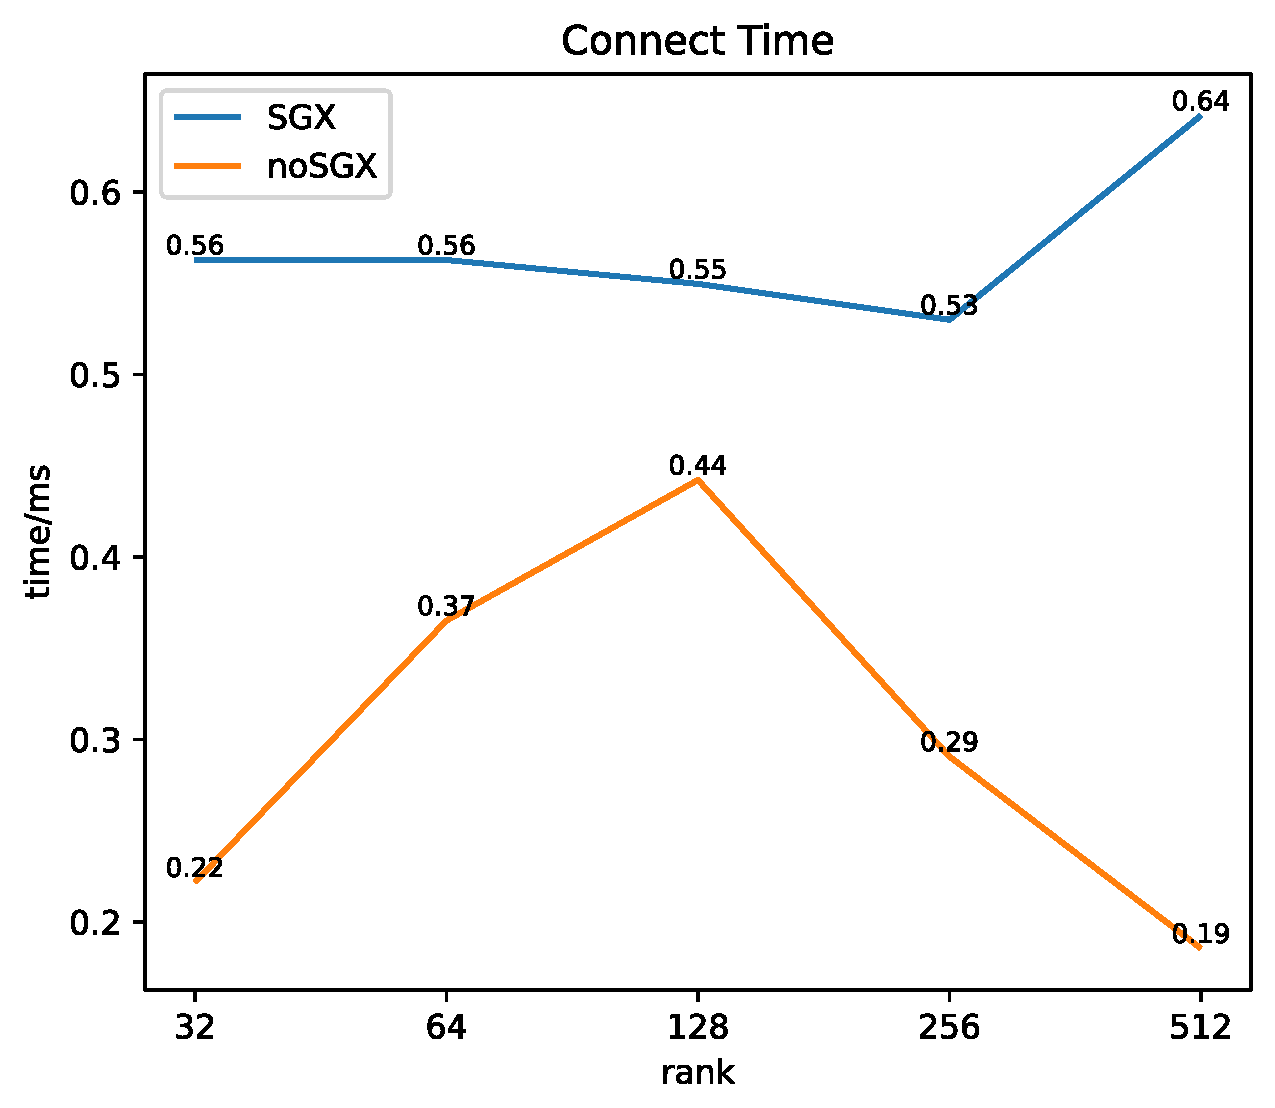
\includegraphics[width=\textwidth]{figures/matrix_connect.pdf}
        \caption{建立TCP连接}
    \end{subfigure}
    \begin{subfigure}{0.4\textwidth}
        \centering
        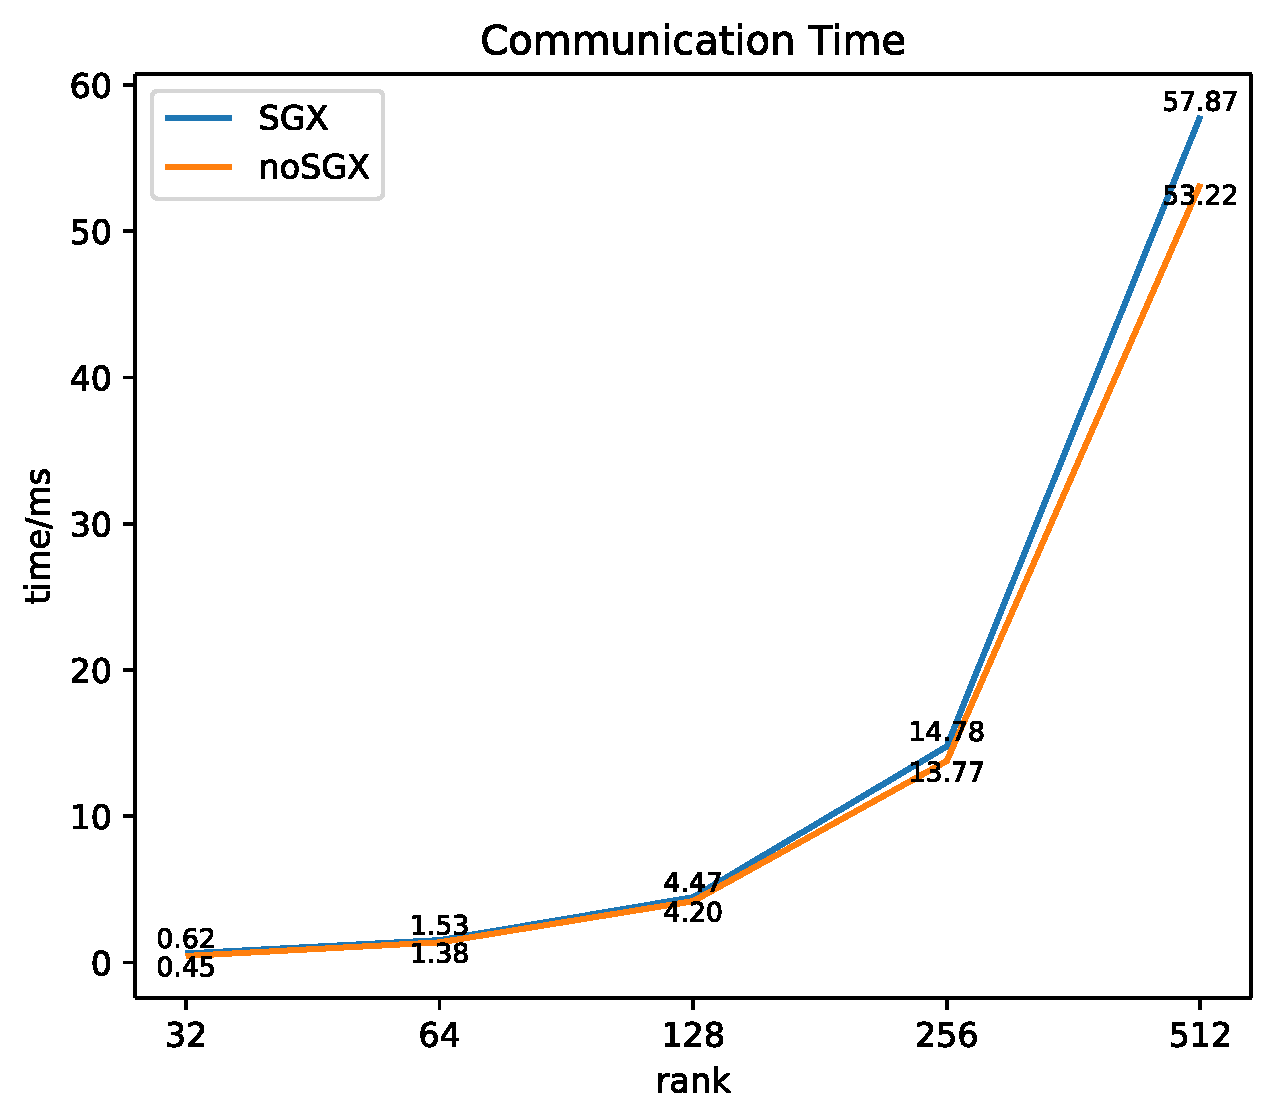
\includegraphics[width=\textwidth]{figures/matrix_communication.pdf}
        \caption{网络通信}
    \end{subfigure}
    \begin{subfigure}{0.4\textwidth}
        \centering
        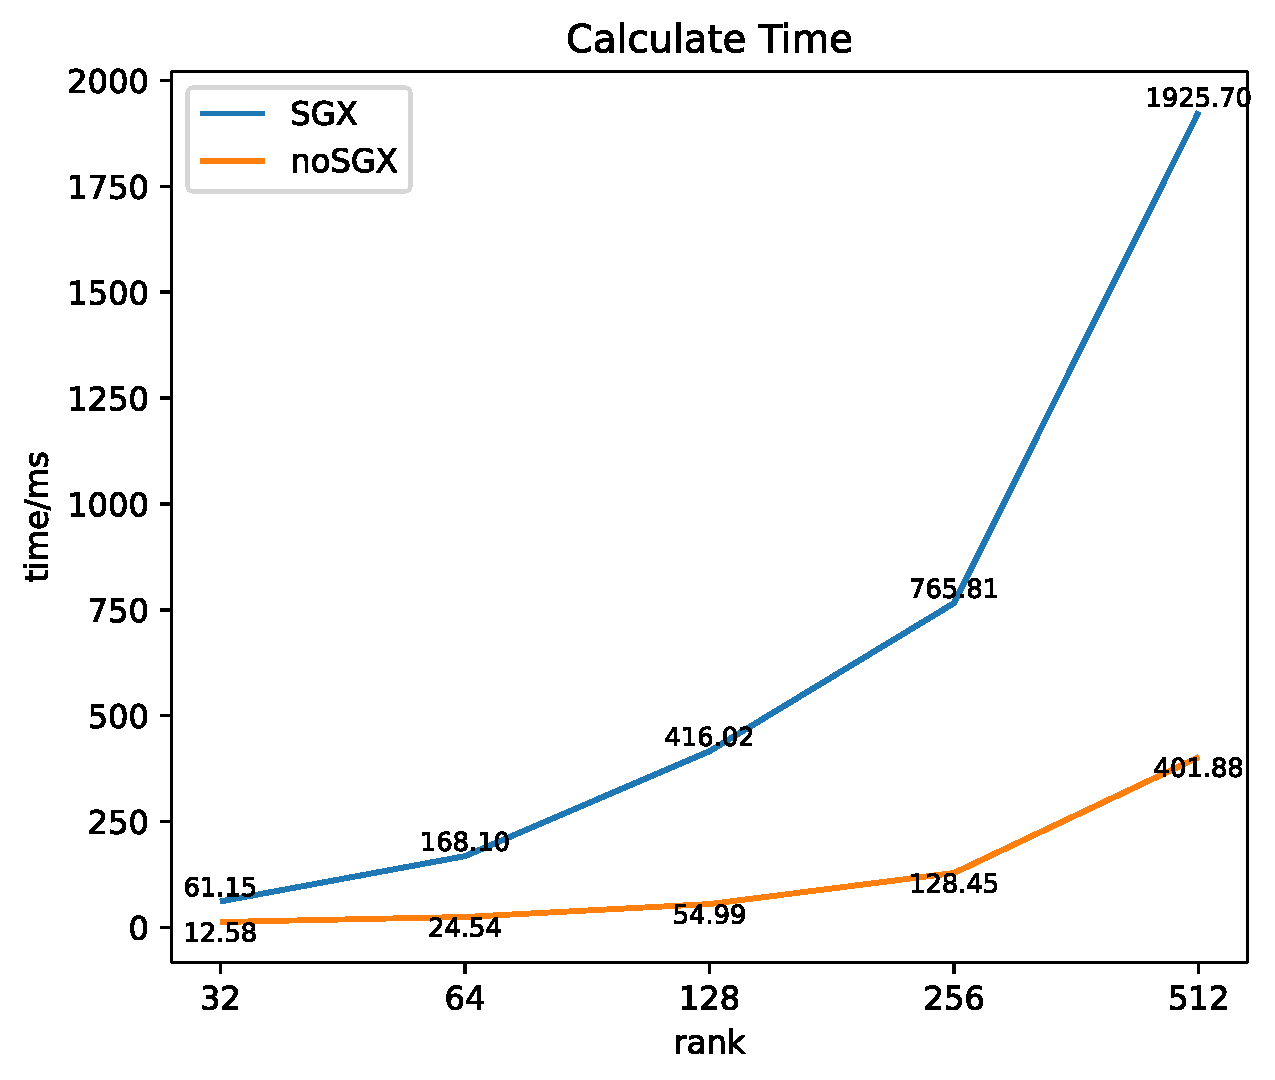
\includegraphics[width=\textwidth]{figures/matrix_calculate.pdf}
        \caption{矩阵计算}
    \end{subfigure}
    \begin{subfigure}{0.4\textwidth}
        \centering
        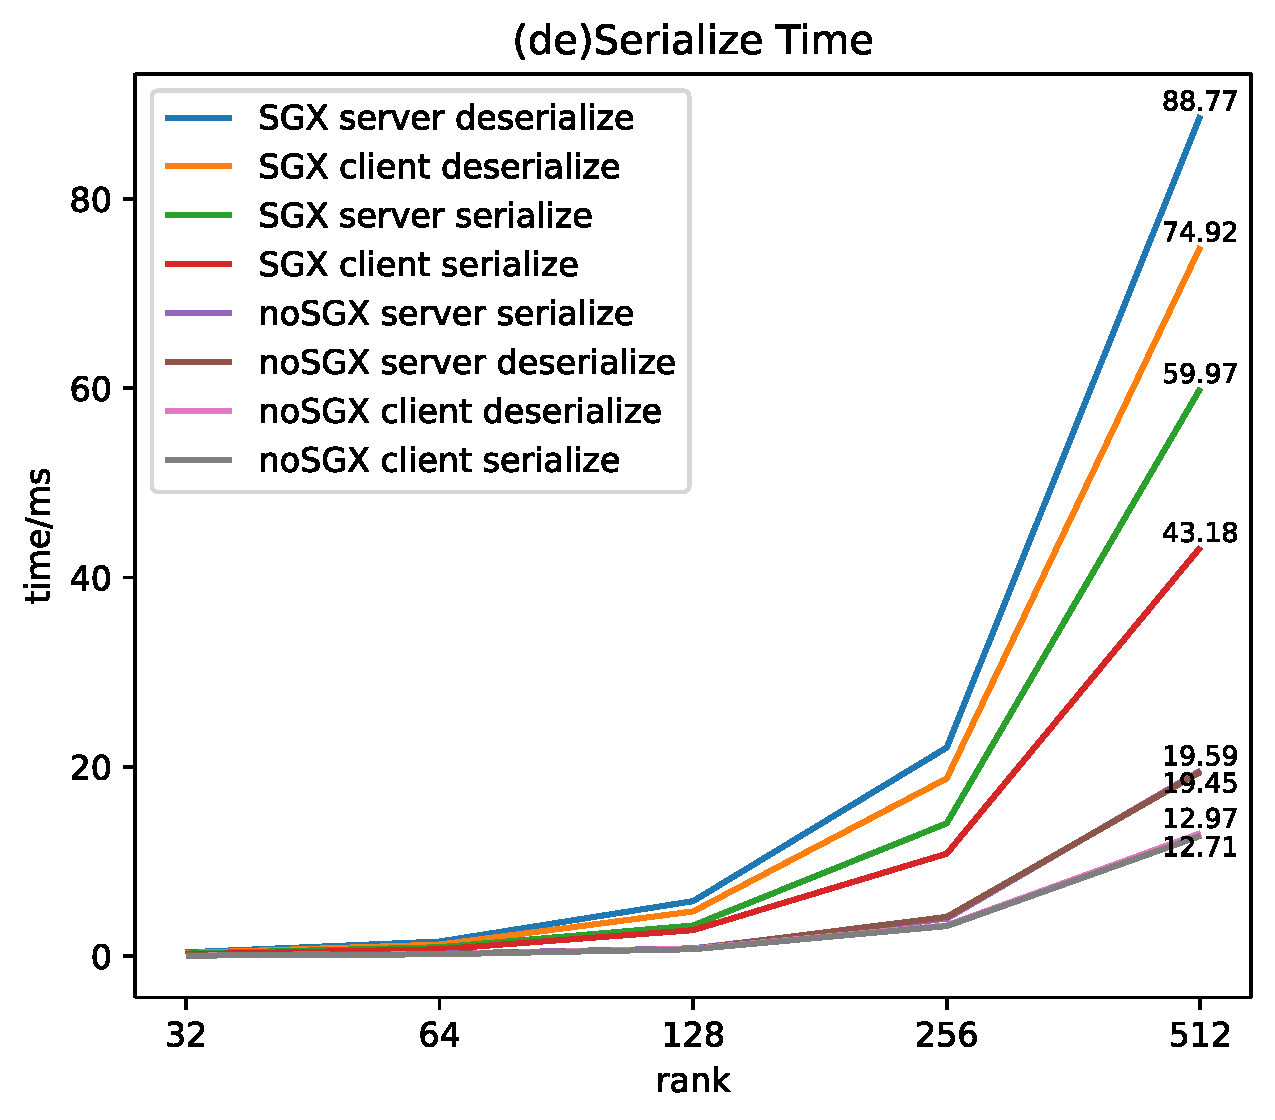
\includegraphics[width=\textwidth]{figures/matrix_serialize.pdf}
        \caption{序列化和反序列化}
    \end{subfigure}
    \caption{RPC各部分耗时}
    \label{fig:matrix-evaluation}
\end{figure}

如图\ref{fig:matrix-evaluation}所示,我们将RPC的耗时分为建立TCP连接、网络通信、矩阵计算、序列化和反序列化共4个不同的开销部分,分别在服务端和客户端对阶为32、64、128、256、512的随机方阵测量耗时。对于建立TCP连接部分,虽然有波动,但基本和数据量大小没有关系;然而跨SGX的延迟是SGX外的1.25-3.37倍。对于网络通信部分,跨SGX通信开销是SGX外的1.14倍左右。对于矩阵计算开销,SGX内的计算约为SGX外的6.01倍。对于序列化和反序列化开销,可以看到数据的明显分层,即SGX服务端反序列化>SGX客户端反序列化>SGX服务端序列化>SGX客户端序列化>非SGX服务端反序列化$\approx$非SGX服务端序列化>非SGX客户端反序列化$\approx$非SGX客户端序列化;总体来说,这一部分也属于计算部分,SGX内的开销约是SGX外的3.40-4.62倍。

综合来看,在本次设计中,通信带来的额外开销较小,但计算的额外开销较大,需要进一步优化。

\subsubsection{安全分析}

如~\cref{subsec:threat-model}讲述的威胁模型所示,本次研究主要针对的攻击手段包括系统特权态攻击、网络攻击、漏洞利用攻击等攻击手段,重点防御隐私泄露问题,结合信任模型,我们可以得到如下的安全性分析:

\begin{itemize}
    \item \textbf{系统特权态攻击}:因为硬件和SGX是可信的,因此根据SGX的防御模型,即使OS或Hypervisor是恶意的或被劫持,SGX中的数据也不会泄露,因此本平台可以防御系统特权态攻击。
    \item \textbf{中间人攻击}:对于中间人攻击,我们使用了DHKE协议来协商对称共享密钥,用以加密保证通信的安全性;即使所有的DH共享参数都被中间人截获,中间人也无法得到密钥,因此无法解读加密信息。同时通过使用SGX远程验证,可以验证微服务节点身份的真实性,防止中间人伪造节点进行攻击。
    \item \textbf{重放攻击}:对于重放攻击,我们在通信协议中加入了计数器,且借助SGX和微服务计算场景的特点,消除了TLS 0-RTT状态恢复情况的漏洞,可以成功过滤掉重放攻击。
    \item \textbf{内存攻击}:对于系统编程语言容易出现的悬垂指针、缓冲区溢出等漏洞带来的内存攻击,我们选择使用安全编程语言Rust,结合其强大的静态分析能力,基本可以消除这些漏洞(除非使用unsafe)。
    \item \textbf{权限扩散}:我们使用JWT的方法进行授权管理,类似于基于功能(Capability)的思想,为了防止权限扩散到下级节点,我们使用了Token交换的授权管理方法,可以实现细粒度的授权管理,减少隐私扩散。
\end{itemize}

另外,在一个完善的微服务场景中,还可能存在物理攻击、DDoS攻击、针对数据库的攻击等,但是针对这些攻击的应对措施与本次研究是正交的领域,因此不在本次研究的讨论范围内。
